\chapter{Harmonogram pracy}

Na poniższych rysunkach przedstawiono harmonogram pracy nad projektem. 
Podział pracy:
\begin{itemize}
    \item Maciej Ejduk - generowanie terenu, generowanie fauny, algorytmy zachowania fauny, skanowanie flory i fauny, budowanie schronienia, cykl dnia i~nocy testowanie, dokumentacja
    \item Mateusz Adamiec - generowanie flory, przygotowanie zbioru modeli, algorytmy zachowania fauny, skanowanie flory i fauny, mechanizmy wskaźników, testowanie
    \item Aleksandra Gajda - przygotowanie zbioru modeli, przygotowanie HUD, zbieranie surowców, mechanizmy wskaźników, poruszanie się, testowanie
\end{itemize}
Skróty w harmonogramie oznaczają osoby odpowiedzialne za wykonanie danego zadania w danym okresie. Ze względu na niedostępność niektórych osób w danych terminach zadanie może posiadać różne składy osób wykonujących dane zadanie w podanych terminach.
\begin{itemize}
    \item MA - Mateusz Adamiec
    \item ME - Maciej Ejduk
    \item AG - Aleksandra Gajda
\end{itemize}


\begin{center}
    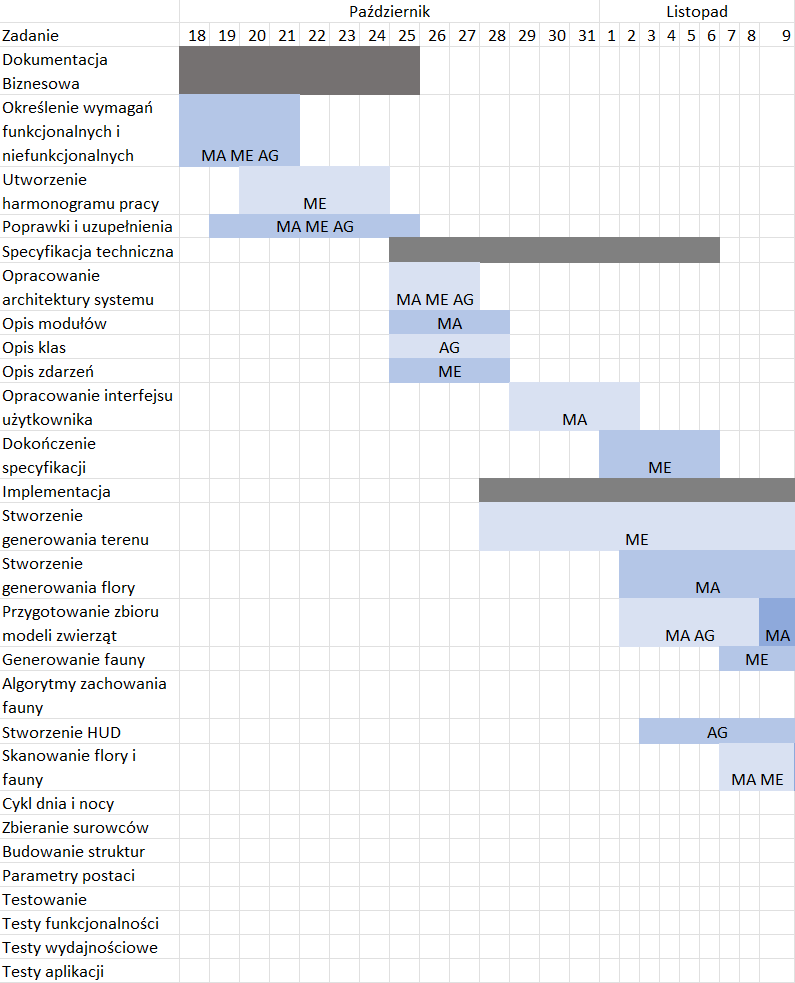
\includegraphics[width=\textwidth]{Graphics/h1.png}
\end{center}

\begin{center}
    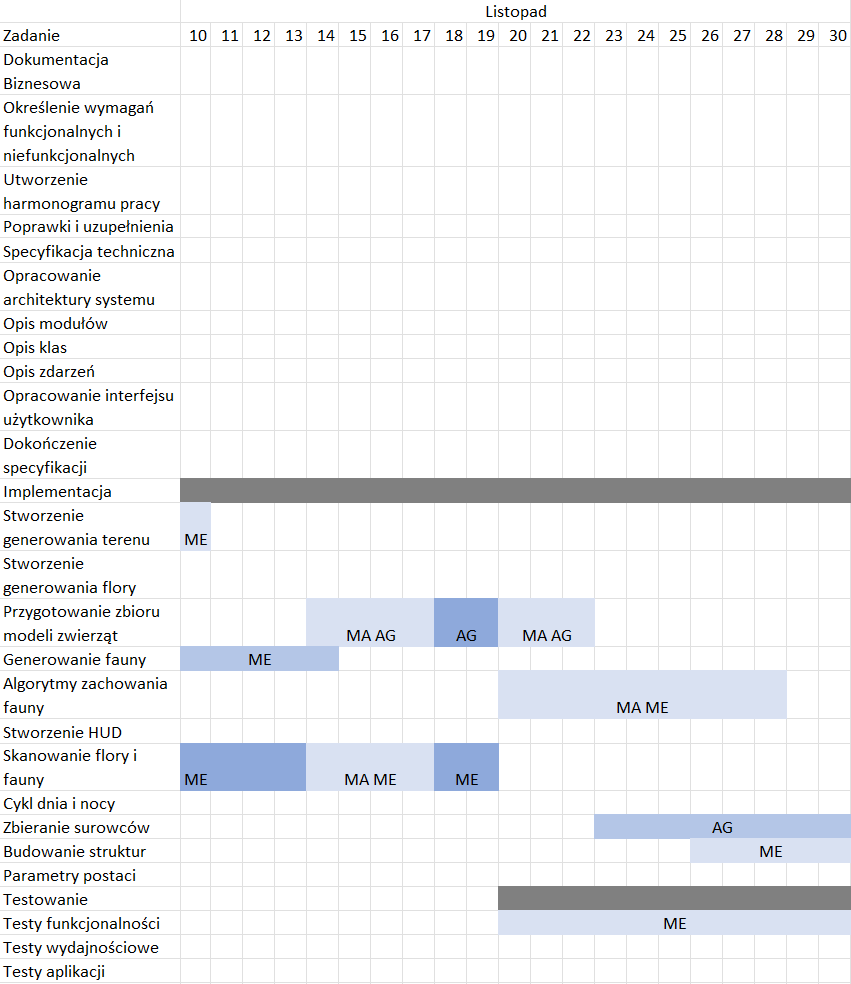
\includegraphics[width=\textwidth]{Graphics/h2.png}
\end{center}

\begin{center}
    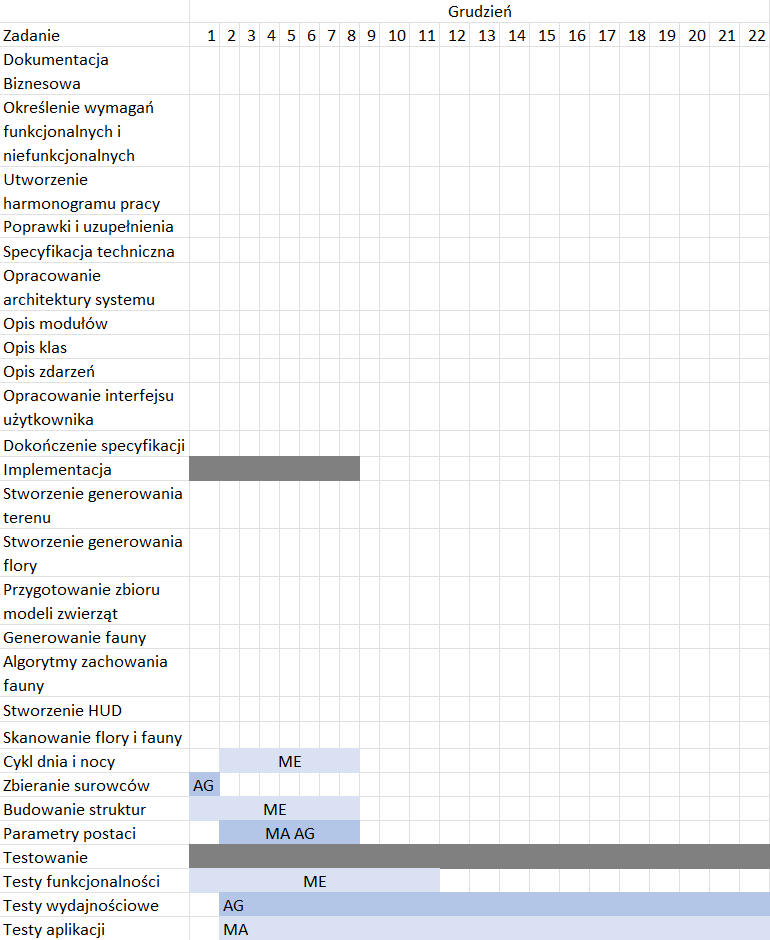
\includegraphics[width=\textwidth]{Graphics/h3.png}
\end{center}